\documentclass[output=paper]{langsci/langscibook} 

\title{Do semantic features capture a syntactic classification of compounds? Insights from compositional distributional semantics} 

\author{%
 Sandro Pezzelle\affiliation{CIMeC -- Center for Mind/Brain Sciences, University of Trento}\lastand
 Marco Marelli\affiliation{Department of Psychology, University of Milano-Bicocca}
}

%\chapterDOI{} %will be filled in at production

% \epigram{}

\abstract{
Classifying compound words has been the ultimate goal of much research in formal linguistics. A popular, cross-linguistically applicable classification \citep{SB2005} distinguishes three main types of compounds, namely Subordinate, Attributive, and Coordinate on the basis of the underlying \textit{syntactic} relation between the compound elements. Similar tripartitions have also been proposed in cognitive psychology by works exploring conceptual combination. Focusing on the type of \textit{semantic} interpretation assigned to novel combinations, three main classes have been traditionally described, namely Relation-linking, Property-mapping, and Hybrid or Conjunctive (see \citealt{wisniewski1996}). Based on these commonalities, we conjecture that syntax-based compound types might also be explained by means of the semantic properties of the compound and its constituents. Using a compositional model of distributional semantics (cDSM), we show that (a) the contribution of each constituent in determining the meaning of the compound and (b) the semantic similarity between the two constituent words are significant predictors of these classes. These findings suggest that the various compound types identified by syntactic criteria can also be predicted by means of semantic features. On the one hand, this confirms the validity of the proposed linguistic categorization. On the other hand, we bring further evidence proving the effectiveness of cDSMs in describing linguistic phenomena.}

\shorttitlerunninghead{Do semantic features capture a syntactic classification of compounds?}
\begin{document}
\maketitle

\section{Introduction}
\label{sec:introduction}

\subsection{Classifying compounds}\label{sec:class}

%\todo{We thank the reviewer for all the insightful comments. Note: We highlight the new text in red, and the changes made to account for reviewer's comments are signalled with a margin note.} 

Compounding, namely the mechanism by which two independent words (e.g. \emph{pet}, \emph{food}) combine together to form a novel morphologically-complex word (e.g. \emph{petfood}), is one of the most extensively covered topics in the literature of word formation.\footnote{For a complete and exhaustive overview of compounding, see \cite{OHC}.} On the theoretical level, many linguists have been particularly interested in classifying \emph{compounds} according to various criteria, such as `headedness' (roughly speaking, the position and the characteristics of the compound \emph{head}, the dominant word in the compound, e.g. \emph{food} in \emph{petfood}) \citep{Bloomfield1933,fabb1998}; the presence of a verb or a deverbal noun \citep{marchand1969}; the kind of underlying relation between the \emph{constituent} words, either at a syntactic level \citep{Bloomfield1933,bally1950,lees1960,SB2005,baroni2006,dressler2006,sbOHC} or at a semantic level \citep{levi1978,warren1978,fanselow1981}. Though different and pertaining to somehow diverse levels of analysis, these criteria have been traditionally explored and mixed together within the same classification framework (see among others \citealt{bauer2001,hasp2002,Booij2005}). As a consequence, many influential proposals distinguish various classes of compounds on the basis of several overlapping properties that often generate an inconvenient number of subclasses and special cases.

To overcome this issue, \cite{SB2005} proposed a cross-linguistic (and nowadays widely accepted) classification framework based on a single, homogeneous criterion, that is, the underlying syntactic relation between the compound constituents. Three main classes of compounds are isolated, namely Subordinate, Attributive, and Coordinate. To illustrate, the compound \emph{doghouse} belongs to the Subordinate class, since the syntactic relation subtending \emph{dog} and \emph{house} is that of subordination. Indeed, the compound can be paraphrased as `the house of the dog'. In contrast, \emph{swordfish} is labeled as Attributive, given that the first constituent, \emph{sword}, acts as an attribute of \emph{fish} (a \emph{swordfish} is `a fish whose nose is shaped like a sword'). Finally, Coordinate compounds are formations like \emph{comedy-drama}, where the first and the second constituent are linked by the underlying conjunction `and'.

\subsection{From \emph{word} combination to \emph{conceptual} combination}

Interestingly, a similar tripartition has been proposed in the cognitive psychology literature by works on \emph{conceptual combination} \citep{wisniewski1996,costello2000}, where the focus is on the type of interpretations provided by people to novel combinations. By analyzing the circumlocutions produced by speakers to interpret novel compounds like \emph{zebra-horse}, in fact, three main classes have been traditionally isolated, namely Relation-linking, Property-mapping, and Hybrid or Conjunctive. The first class includes interpretations involving a relation between the two concepts, i.e. a \emph{zebra-horse} is `a horse that preys zebras'. In the second, a property of one concept is mapped to the other, i.e. a \emph{zebra-horse} is `a striped horse'. In the third, the novel concept is interpreted as a hybrid or conjunction of the constituent concepts, i.e. a \emph{zebra-horse} is `a creature having many properties of both horses and zebras'. Though the aim of these works is to study the various interpretations to novel conceptual combinations, without any interest in recognizing classes of \emph{lexicalized} compound words, the types they identify are reasonably comparable to the linguistic ones proposed by \cite{SB2005}. In particular, Relation-linking interpretations correspond to compounds included in the Subordinate class, Property-mapping to Attribute, and Hybrid/Conjunctive to Coordinate.

A notable difference is that the \emph{linguistic} classification accounts for lexicalized (or familiar) compounds, whereas the \emph{cognitive} one describes novel combinations which still lack a single, well-defined interpretation. However, we can easily assume that lexicalized compounds are the linguistic realization of a conceptual combination process, in a way that all compounds start out as novel formations and become lexicalized with usage in time \citep{gagne2006}. Consistent with this claim is recent evidence showing that, in the processing of both novel and familiar compounds, an active combination of constituent meanings is routinely in place \citep{gagnesp2009,ji2011,marelli2012,marelli2014}. This would suggest that the difference between novel and familiar compounds is merely in their degree of lexicalization. While the former can still be interpreted by speakers in various ways, the latter have only one possible interpretation, that the classification by \cite{SB2005} describes in terms of a fixed syntactic relation between the compound's constituents.

%that corresponds to a fixed syntactic relation between the constituent words in \cite{SB2005}.

%It should be mentioned at this point that the position about compositionality in compounding is not unanimous among theorists. That is, although linguists generally agree in considering compounds as the result of some kind of composition of two (or more) words, there is no consensus on what compositionality means when referred to compounds. \cite{libben2014}, for example, argues that the meaning of a compound is extremely rarely determined by the meanings of its constituents. Similarly, \cite{dressler2006} assumes that, due to lexicalization, compounds are never fully transparent in the sense of Frege's Principle of compositionality. More generally, it is often claimed that the meaning of a complex word represents something more than the simple addition of the parts. Similar claims can be found in the literature on conceptual combination, with \cite{gagne2006} arguing that understanding a combined concept involves creating a new concept rather than interpreting the whole as a sum or hybrid of the parts. However, a certain degree of compositionality can be found even in fully opaque compounds (e.g., butterfly), whose meaning is the result of a process of lexicalization that darkened their original, fully-compositional meaning (see \cite{marelli2015}).

The second important difference is that interpretations of novel combinations pertain to the conceptual level, that is, they describe relations between the concepts being combined together. As such, the tripartition described above is essentially \emph{semantic}. In contrast, the linguistic classification considered here is based on a purely \emph{syntactic} criterion. Based on the commonalities highlighted above, however, it might be that the two levels of analysis are not mutually exclusive, but possibly related and somehow overlapping. Lexical semantic approaches corroborate this conjecture. \cite{lieber5OHC}, for example, proposed that the different compound types identified by \cite{SB2005} depend, at least in part, on the intrinsic semantic features of the compound constituents. Moreover, classifications of compounds based on taxonomies of semantic relations reveal a certain degree of overlap between the syntactic and the semantic analysis \citep{levi1978}. For example, the semantic relation \texttt{AND} seems hardly distinguishable from the purely syntactic relation of coordination, which is subtended by the underlying conjunction `and'.

\subsection{Aim of the work}

Based on this concurring evidence, we conjecture that various classes of compounds defined at the syntactic level may be also explained in terms of the semantic properties of the compounds and their constituents. In particular, our hypothesis is that measures quantifying the semantic role played by each constituent in contributing to the overall compound meaning, as well as the degree of semantic similarity between the constituents, should be effective in predicting different classes. Moreover, we expect these semantic measures to be able to capture different, syntax-based classes without relying on other non-semantic properties of compounds. Crucially, we do not claim that the distinction is thus purely semantic, making superfluous any categorization focusing on the syntactic relation between the compound constituents. Rather, we believe that the theoretically motivated and widely accepted \emph{discrete} classifications proposed by linguists can be also described in terms of the \emph{continuous}, quantitative aspects of the meaning of compounds and their constituents. In other words, we expect the \emph{quantitative} semantic properties to parallel the \emph{qualitative} grammatical distinctions, thus demonstrating, at the same time, the effectiveness of our proposal and the validity of the linguistic theory.

We experiment with a dataset of English compounds for which annotation based on the classification by \cite{SB2005} (Subordinate, Attributive, Coordinate) is available. To predict each class, we use several semantic variables such as the degree of similarity between the constituents and the individual contribution of each constituent word in determining the meaning of the whole compound. We quantify these measures by using a compositional model of distributional semantics \citep{baroni2010,guevara2010,mitchell2010,zanzotto2010}, following recent evidence proving the effectiveness of this approach in modeling morphological processes such as composition and derivation \citep{marelli2015,gunther2016,marelli2017}.

\subsection{Computational models of meaning}

Based on the core notion that similar words occur in similar contexts \citep{harris1954,firth1957}, distributional semantic models (henceforth, DSMs) represent lexical meanings by means of vectors encoding the contexts in which words appear in a large corpus. The intuition is that words that occur in similar linguistic contexts (e.g., \emph{cat} and \emph{dog}) should be semantically more similar than words that do not. Typically, this geometric representation is used to quantify the degree of distributional similarity between two words. Given the corresponding vectors, the similarity is computed in terms of their geometric distance, typically the cosine of the angle \citep{turney2010}. In particular, the closer two vectors in the semantic space (i.e., the space populated by all the linguistic vectors), the higher their similarity. Traditional DSMs, such as the pioneering Latent Semantic Analysis (LSA; \citealt{landauer1997}), have been largely used to obtain quantitative estimates of important semantic variables such as the degree of conceptual or topical similarity between two words \citep{pado2007,gagnesp2009,kuperman2009,wang2014}.

%\todo{We added a new subsection where distributional semantic approaches to compound interpretation and compositionality prediction are discussed.}

\subsection{Distributional semantics and compounds}\label{sec:relnew}

In the domain of compounds, distributional semantic approaches have been extensively applied to two main tasks: noun-noun compound interpretation~\citep{van2013melodi,dima2015automatic,dima2016compositionality,P18-1111,fares2018transfer} and compositionality prediction~\citep{reddy2011empirical,im2013exploring,salehi2014using,salehi2015word,cordeiro2016predicting}. The former task, usually tackled as a classification problem, aims at automatically predicting the \emph{semantic} interpretation of the compound (i.e., the semantic relation between the constituents). Given the compound \emph{street protest}, for example, a system is trained to predict that the relation holding between the nouns is `locative'. Several datasets of compounds annotated with different numbers of semantic relations have been released for the tasks~\citep{o2007annotating,tratz2010taxonomy}, and various systems capitalizing on distributional representations (usually obtained with neural network architectures; see section~\ref{sec:vectors}) have been recently proposed. Overall, this approach has been proved to be successful in the task, though the performance is shown to be dependent on the number and granularity of semantic relations. As for the latter task, it is focused on predicting the degree of compositionality of a noun-noun compound, namely the extent to which the meaning of the whole depends on the meaning of the constituent words. Various datasets annotated with human judgments have been proposed through time~\citep{reddy2011empirical,roller2013expected,farahmand2015multiword}, and extensive explorations of DSMs in the task have been carried out. Crucially for the purpose of this study, distributional measures of similarity obtained with compositional approaches were found to be highly predictive of human judgments in this task~\citep{reddy2011empirical,im2013exploring,salehi2015word,cordeiro2016predicting}.

\subsection{A compositional approach to compounds}\label{sec:compapp}

Of great interest for the present work, \cite{lynott2001} were the first to employ distributional semantic models to study novel compounds (e.g. \emph{zebra-horse}). In particular, the aim of that work was to test whether a measure of semantic similarity between compound constituents (quantified with LSA) was predictive of both (a) the ease of novel compound comprehension and (b) the distinction between Relation-linking and Property-mapping combinations. To do so, they experimented with novel compounds and their corresponding interpretations as provided by previous works on conceptual combination \citep{wisniewskilove,gagne2000}. Overall, the model was shown to perform remarkably well in all the tasks. \cite{lynott2001}, however, claimed that current distributional models like LSA were not capable of modeling the whole process of conceptual combination. Since they can only quantify the similarity between independent, free-standing words (e.g. \emph{zebra} and \emph{horse}), they are not informative at all about the relation between these words and the resulting compound. As such, they represent static, word-based models of lexical semantics which do not account for the potentially infinite linguistic productivity.


Compositional DSMs (hence, cDSMs) tackle precisely these issues. Aimed at accounting for the compositional nature of language \citep{baronifrege}, these models capitalize on DSM vectors and perform either simple \citep{mitchell2010} or more complex, theoretically inspired operations \citep{baroni2010,guevara2010,zanzotto2010} to \emph{compose} existing lexical entries. By exploiting simple operations (sum, multiplication) or being trained with distributional information about combinations that are already observed in the source corpus, these models can indeed be used to generate meaning representations for both novel and lexicalized formations. Recently, this approach was shown to be effective in modeling morphological processes such as derivation and compounding \citep{marelli2015,gunther2016,marelli2017}. Closely related to the present study, recent work \citep{gunther2016,marelli2017} exploited cDSMs to generate compositional representations of compounds. \cite{marelli2017}, in particular, explored whether a simple but effective regression-based compositional method \citep{guevara2010} can capture the variability in semantic relations between the constituents of novel compounds. This system was shown to be remarkably effective and flexible in capturing relational information. Based on this evidence, in the present work we employ the same model and test it in the task of predicting theoretically motivated, syntax-based classes of compounds.

%The paper is structured as follows: First, we introduce the method, the materials, and the variables used for testing our hypothesis. Then we present the results by means of in-depth analyses. Finally, we discuss the results and discuss their implications. 

\section{Experiment}
\label{sec:experiments}

The present experiment investigates whether different, syntax-based classes of compound words (Subordinate, Attributive, and Coordinate) can be captured by means of semantic properties of the compound and its constituents. To quantify these properties, (a) we generate compositional representations of compounds and obtain similarity scores assessing the role of each constituent in contributing to the overall meaning; (b) we measure the degree of similarity between the first and second constituent.

A note on the terminology used in the paper. Until this point, we used the neutral terms `first constituent' and `second constituent' to refer to, respectively, \emph{dog} and \emph{house} in \emph{doghouse}. As briefly mentioned in section \ref{sec:class}, one constituent usually plays a dominant role compared to the other since it acts as the `head' of underlying phrase. In this example, the head is clearly \emph{house} (indeed, \emph{doghouse} is `the house of the dog'). Consistently, this element determines the syntactic category of the phrase and, semantically, it represents a hyperonym of the compound. By default, in English compounds the second constituent acts as the compound `head', whereas the first acts as the compound `modifier' \citep{bauerOHC}. We stick with this arguably simplified terminology\footnote{Without going into much detail, it should be mentioned that this picture is indeed less straightforward than it may appear. For instance, in the English compound \emph{singer-songwriter} the two constituents play a similar role, in a way that they could be both considered as the compound `head' (and the compound as `double-headed') \citep{bauerOHC}.} and, from now on, we interchangeably use the terms `first constituent' or `modifier' to refer to the leftmost element, `second constituent' or `head' to refer to the rightmost one.


\subsection{Semantic space}\label{sec:vectors}

Following \cite{baronipredict}, who demonstrated that DSMs generated using feedforward neural network models largely outperform traditional count-based architectures in many tasks, we built a state-of-the-art \texttt{CBOW} semantic space using the \texttt{word2vec} toolkit by \cite{mikolov2013}, with all the parameters that turned out to be best-predictive in \cite{baronipredict}. In particular, the vectors have 400 dimensions and were built using (a) a context window of 5 words to either side of the target word, (b) a subsampling procedure which penalizes high-frequency words in the training phase (t = 1\emph{e}\textsuperscript{-5}), (c) 10 negative samples. The vectors were trained using a corpus of written English containing around 2.8-billion tokens (a concatenation of BNC, ukWaC, and a 2009-dump of Wikipedia), the same used in \cite{baronipredict}. To avoid sparsity effects, we experimented with the vectors corresponding to the 300K most frequent words in the corpus.


\subsection{Materials}

We experimented with a sample of the MorBoComp database including 163 English compounds. MorboComp is a large, multilingual database of compounds that has been developed to study compounding from a typological perspective.\footnote{For further details, see: \url{http://morbocomp.sslmit.unibo.it/index.php?section=home}} Each compound in the database is richly annotated (i.e., it is provided with information about headedness, compound and constituents' grammatical category, compound structure, etc.) and, crucially for our purposes, it is classified as Subordinate (hence, SUB), Attributive (hence, ATT) or Coordinate (hence, CRD) on the basis of the classification and terminology proposed by \cite{SB2005}. To illustrate, \emph{schoolteacher} is tagged as SUB, \emph{keyword} as ATT, and \emph{king-emperor} as CRD.

Consistent with the criteria outlined in \cite{SB2005}, the 163-item sample contained cases of both `phrasal' compounds (\emph{do-it-yourself illustration}, \emph{around-the-world flight}) and `neoclassical' formations (\emph{bibliography}, \emph{theology}). In addition, a handful of items labeled with OTH (i.e., Other) were found. However, since this label was used by the annotators for either unresolved or idiosyncratic cases, we decided not to consider them in our investigation. Similarly, we removed neoclassical formations since their constituents can be affixes and suffixes rather than free-standing, independent words (e.g. \emph{biblio-}). As a consequence, in our distributional semantics approach we could not have a vector representation for these items. Finally, additional 9 compounds were discarded since one of their constituents turned out not to be included in the 300K-vector semantic space. Specifically, 8 out of 9 of the missing items were first constituents of phrasal compounds, e.g. \emph{all-goes-well} (\emph{in all-goes-well atmosphere}) or \emph{floor-of-a-birdcage} (\emph{in floor-of-a-birdcage taste}), whereas in one case (\emph{well-deserver}) the missing items was the second constituent (\emph{deserver}). After this filtering process, our resulting dataset included 132 compounds (67 SUB, 49 ATT, 16 CRD), that we used for our experiment.


\subsection{Generating composed representations}


For each of the 132 compounds in the list, we generated a composed representation using the vectors described in section \ref{sec:vectors} and the compositional model by \cite{guevara2010}. As previously mentioned, one of the main strengths of compositional DSMs is their ability to produce meaning representations also for combinations that are not attested in the source corpus. That is, given a novel or unattested compound, we are able to represent it as an independent vector on the basis of the meanings of its constituents (\emph{zebra} and \emph{horse}). This aspect was of crucial importance in our experiment, where 60 out of the 132 compounds extracted from MorBoComp turned out not to be present in the source semantic space. That is, almost half of the compounds were not among the 300K most frequent words in the corpus and, consequently, did not have a distributional representation. By using a compositional model capitalizing on the representations of the two constituents, however, we were able to overcome this limitation of traditional DSMs and generate a meaning representation for all the items, regardless of whether they had a `static' semantic representation or not.



The method used in the present study, in particular, was implemented by \cite{guevara2010} to model compositionality as depending on the semantic relation instantiated in the syntactic structure. As such, it looks particularly suitable for the case of compounds, which embed a modifier-head structure. Indeed, previous work proved this model to be very effective in generating composed representations for compounds \citep{marelli2017}. Technically, the composed representations are obtained with the combinatorial procedure depicted in Figure~\ref{fig:caoss}: given two vectors \(\overrightarrow{u}\) and \(\overrightarrow{v}\) each representing one of the constituent words, their composed representation can be computed as \(\overrightarrow{c}\) = \textbf{M}\(\overrightarrow{u}\) + \textbf{H}\(\overrightarrow{v}\), where \textbf{M} and \textbf{H} are weight matrices estimated from training examples. These matrices are trained using least squares regression,\footnote{As reported by \cite{guevara2010}, this method is commonly employed to approximate functions in problems of multivariate multiple regression with a small number of observations and a greater number of variables, that is a similar condition to the one involving high-dimensionality vectors representing word meanings and (relatively) limited data.} having the vectors of the constituents as independent words (\textit{dog}, \textit{house}) as inputs and the vectors of example compounds (\textit{doghouse}) as outputs. The two matrices are thus optimized so that the similarity between the weighted sum of the two constituent vectors (the composed vector) and the compound vector extracted from the semantic space (the observed vector) is maximized. Or, in other words, the composed vector obtained by means of the compositional model is built in a way that closely approximates the original one.


\begin{figure}[t!]
\begin{center}
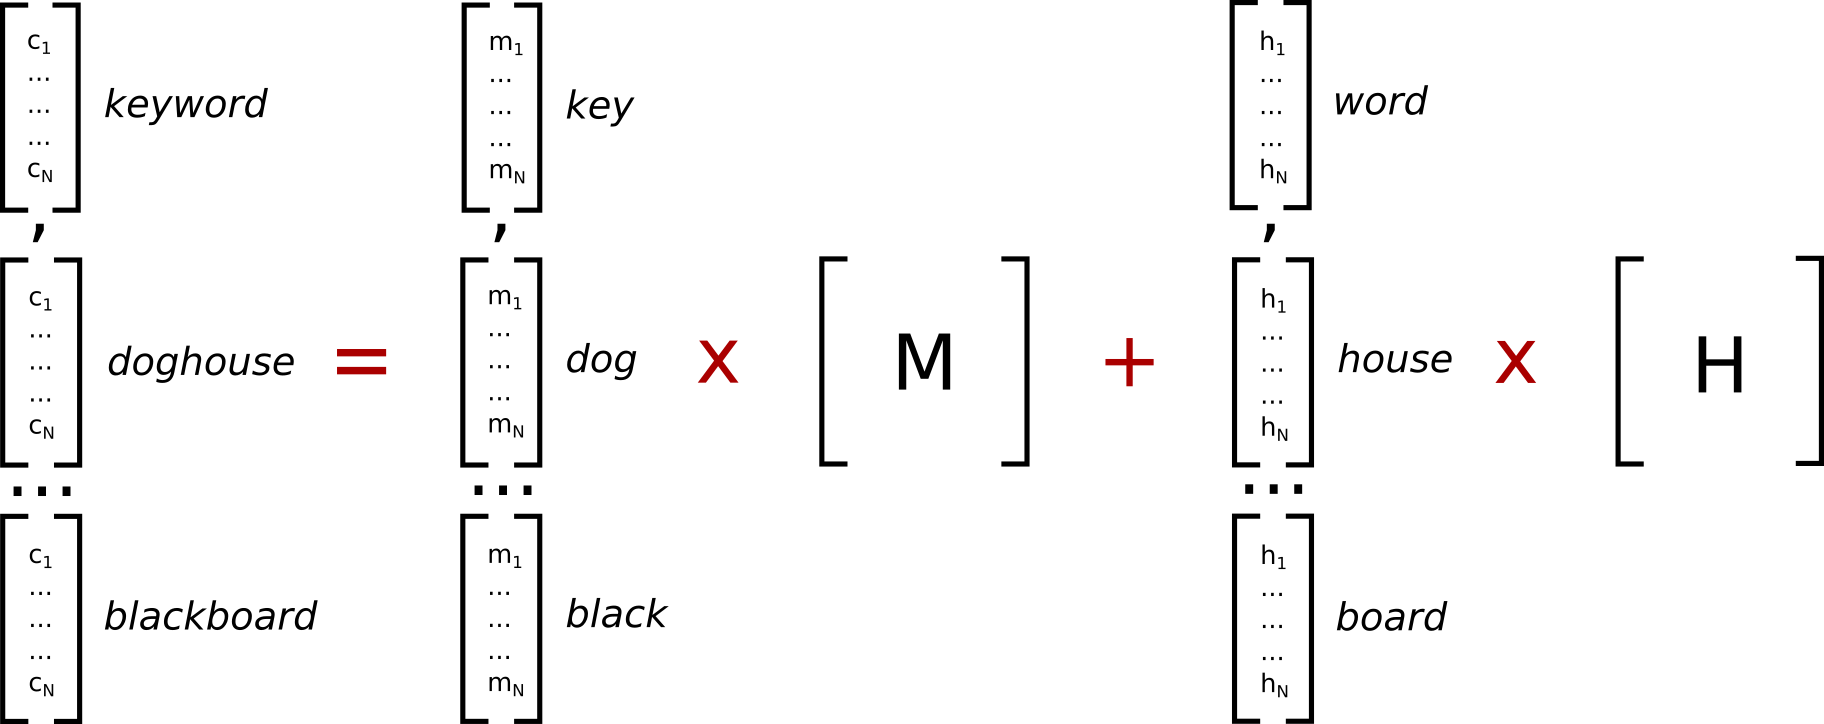
\includegraphics[width=0.9\textwidth]{figures/plsr1.png}
\caption{Representation of the training phase of the compositional method used in the study (adapted from~\citealt{marelli2017}).}\label{fig:caoss}
\end{center}
\end{figure}




In the present study, we trained the compositional model with a list of English noun-noun compounds extracted from the CELEX English Lexical Database \citep{celex}. By default, we treated all compounds as written in \emph{solid} form, that is, without whitespaces or hyphens between the two constituents. When the solid compound was not found in our semantic space, we looked for it in its hyphenated form. The training set included 2174 triplets <modifier, head, compound>, none of which was also present in the dataset we obtained from MorBoComp. We then used the estimated weight matrices for generating composed representations for each of the 132 compounds in our sample.


\subsection{Semantic variables}

For each vector obtained compositionally, we computed four composition-based semantic measures, namely (1) similarity between the composed representation of the compound and its modifier (e.g. between \emph{keyword} and \emph{key}), (2) similarity between the composed representation of the compound and its head (e.g. between \emph{keyword} and \emph{word}), (3) neighborhood density, that is, the average cosine similarity between the composed vector and its top-10 nearest neighbor vectors in the semantic space (all these 3 measures have been introduced by \citealt{vecchi2011}), and (4) entropy, that is a measure of vector quality firstly introduced by \cite{lazaridoufish}.

By operationalizing the similarity between the composed compound vector and either constituents, in particular, we aimed at quantifying the extent to which each single word contributes to the overall meaning obtained compositionally. Although operationalized in terms of the cosine of the angle between the compound vector and either constituents (in the same way as standard DSMs do), indeed, these measures genuinely describe the morphological process itself rather than merely taking into account its start and end points. Based on these properties, such measures have been recently used in studies with compound words. For example, they have been shown to be effective in predicting meaningfulness ratings on novel combinations \citep{gunther2016} and in capturing relational information in compounds \citep{marelli2017}.

%contributes to the overall, compositionally-obtained meaning.

As far as neighborhood density and entropy are concerned, both of them have been proposed to provide information about the meaningfulness of vectors encoding new concepts. The rationale of the former is that meaningful vectors should live in a region of the semantic space that is densely populated by vectors representing many related concepts, while meaningless vectors should be way more isolated. For the latter, the intuition is that meaningful vectors should have a skewed distribution, with few dimensions (corresponding to the salient semantic features of the word) being highly activated, i.e. having large values. In contrast, meaningless vectors should have a more uniform distribution, which would be a proxy for a less defined, fuzzier meaning. As a consequence, entropy would be inversely correlated with meaningfulness.

A (5) fifth semantic but non-compositional measure was introduced following \cite{lynott2001}, who employed Latent Semantic Analysis (LSA) to quantify the degree of similarity between the first and the second constituent of a compound. Here, we took the compound constituent vectors (e.g. the vectors of \emph{key} and \emph{word}) from the source semantic space (see section~\ref{sec:vectors}) and simply computed their cosine similarity. This measure might be helpful in distinguishing between different compound classes, based on the evidence that in both theoretical linguistics (see \citealt{lieber5OHC}) and conceptual combination literature (see \citealt{wisniewski1996}) this factor has been considered as explanatory of different classes/interpretations.

\subsection{Non-semantic variables}

In addition to the 5 semantic variables described above, we also included in our experiment a number of non-semantic control variables. For each compound and its constituent words we extracted word-form frequency from the source corpus (i.e., the number of times a word is encountered in the corpus in that exact form, regardless of its grammatical category). Compound frequency was calculated by summing the occurrences of the given compound in both solid and hyphenated orthographic form (\emph{blackboard} and \emph{black-board}, respectively). All frequency values, namely (6) compound frequency, (7) modifier frequency and (8) head frequency were subsequently log-transformed following standard practice in psycholinguistics \citep{brysbaert2018}.


In addition, we computed (9) Pointwise Mutual Information (PMI) between the constituents as a measure of compound lexicalization. This widely-used association measure \citep{church1990} compares the probability of co-occurrence of two words in the source corpus with the probability of the two words co-occurring by chance. To illustrate, although the word pair <the apple> is likely much more frequent than <apple juice>, the PMI of the latter will be higher, since the determiner \emph{the} is likely to co-occur very frequently with any noun in the corpus, thus being less informative compared to the pair <apple juice>, whose mutual association is intuitively strong. In particular, the higher the degree of lexical association between two words, the higher the PMI value.

Finally, we included (10) compound length measured as the number of characters making up the string (e.g., \emph{blackboard} has length 10). When present, hyphens were not counted. Descriptive statistics including mean values and standard deviations for all the predictors used in the present experiment are reported in Table~\ref{tab:descriptives}.

\begin{table}[t]
\resizebox{\textwidth}{!}{\begin{tabular}{l *{8}{S[table-format=2.2]}}
\lsptoprule
Predictor          & \multicolumn{2}{c}{SUB} & \multicolumn{2}{c}{ATT} & \multicolumn{2}{c}{CRD} & \multicolumn{2}{c}{Total}  \\ \cmidrule(lr){2-3}\cmidrule(lr){4-5}\cmidrule(lr){6-7}\cmidrule(lr){8-9}
                   & \textit{mean}   & \textit{sd}   & \textit{mean}    & \textit{sd}   & \textit{mean}   & \textit{sd}   & \textit{mean} & \textit{sd} \\ \midrule
MCsim              & 0.21            & 0.10           & 0.18             & 0.09          & 0.24            & 0.13          & 0.20           & 0.10         \\
HCsim              & 0.25            & 0.11          & 0.21             & 0.10           & 0.24            & 0.10           & 0.23          & 0.11        \\
MHsim              & 0.13            & 0.10           & 0.14             & 0.09          & 0.34            & 0.15          & 0.16          & 0.12        \\
Density            & 0.41            & 0.07          & 0.40              & 0.09          & 0.39            & 0.08          & 0.40           & 0.08        \\
Entropy            & 4.50             & 0.05          & 4.99             & 0.06          & 5.01            & 0.05          & 4.50           & 0.06        \\
Comp length        & 10.40            & 2.54          & 10.90             & 3.37          & 10.90            & 2.94          & 10.70          & 2.90         \\
Comp freq          & 1.87            & 1.17          & 2.25             & 1.38          & 2.31            & 0.72          & 2.06          & 1.22        \\
Mod freq           & 5.26            & 0.86          & 5.31             & 1.38          & 5.32            & 0.48          & 5.29          & 1.05        \\
Head freq          & 4.97            & 0.85          & 4.92             & 0.89          & 5.12            & 0.65          & 4.97          & 0.84        \\
PMI                & 3.53            & 4.00             & 4.83             & 4.80           & 4.34            & 3.47          & 4.11          & 4.27        \\ \midrule
\textit{Num items} & \multicolumn{2}{c}{67}          & \multicolumn{2}{c}{49}          & \multicolumn{2}{c}{16}         & \multicolumn{2}{c}{132}    \\ \lspbottomrule
\end{tabular}}
\caption{Mean and standard deviation of all the predictors included in the experiment. MCsim: modifier-compound similarity. HCsim: head-compound similarity. MHsim: modifier-head similarity. Comp length: compound length. Comp freq: compound frequency. Mod freq: modifier frequency. Head freq: head frequency.}\label{tab:descriptives}
\end{table}

\subsection{Data analysis}


Our hypothesis is that various, syntax-based classes of compounds might be predicted on the basis of semantic features. If this is correct, our semantic variables will turn out to be reliable predictors of one class over the others. In order to test our hypothesis, we included all the predictors reported in Table \ref{tab:descriptives} in a series of logit regression models that individually estimated the probability of one class over the other. That is, we tested three separate models in the task of predicting one compound type against each of the others: (1) ATT vs SUB, (2) ATT vs CRD, (3) CRD vs SUB.

All analyses were carried out within the \texttt{R} statistical computing environment. We adopted a backward procedure to progressively simplify each statistical model. Starting from a full-factorial model including all the independent variables, predictors were removed one by one when their absence did not significantly lower the overall model fit. At each step, the removal procedure was attempted for the predictor with the largest p-value. The contribution of each parameter to be removed was checked with a goodness-of-fit chi-square test. Finally, atypical outliers were identified and removed using as a criterion 2.5 standard deviation of the residual errors.


\section{Results}
\label{sec:results}

%In order to report results in a readable format, we discuss each model in a separate subsection by also providing a table summarizing the results. 

For the better presentation of results, we summarize them in tables and discuss each model in a separate section. In the leftmost part, each table reports the list of variables included in the full-factorial version of each model. In the central part, model-simplification procedure (\emph{Removal order}), chi-square goodness-of-fit test (\emph{Chi-square}) and its results (\emph{p}) are reported. The rightmost part shows the effects of the variables included in the final model.

\begin{table}[t]
\resizebox{\textwidth}{!}{\begin{tabular}{lS[table-format=1.4]S[table-format=1.4]cS[table-format=-1.4]S[table-format=-1.3]S[table-format=1.5]}
\lsptoprule
Parameter            & {Chi-square} & {p}      & Removal order & {Estimate} & {z-value} & {p}      \\ \midrule
(Intercept)                  & {--}       & {--}     & Not removed   & -0.8362  & -0.741  & 0.4587 \\
MCsim & {--}       & {--}     & Not removed   & -6.4337  & -2.361  & 0.0182 \\
HCsim     & {--}       & {--}     & Not removed   & -5.5904  & -2.102  & 0.0355 \\
Density         & {--}       & {--}     & Not removed   & 7.6332   & 1.916   & 0.0553 \\
PMI & {--}       & {--}     & Not removed   & 0.0878   & 1.885   & 0.0594 \\
MHsim     & 2.5275   & 0.1119 & 6             &          &         &        \\
Head freq               & 0.7637   & 0.3822 & 5             &          &         &        \\
Mod freq           & 0.4882   & 0.4847 & 4             &          &         &        \\
Comp length              & 0.8206   & 0.365  & 3             &          &         &        \\
Comp freq           & 0.0745   & 0.7848 & 2             &          &         &        \\
Entropy                      & 0.005    & 0.9433 & 1             &          &         &        \\ \lspbottomrule
\end{tabular}}
\caption{Results of the logit model opposing ATT (1) to SUB (0).\label{tab:resattsub}}
\end{table}

\subsection{ATT vs SUB}

The first model, testing ATT (\emph{halfprice}) against SUB (\emph{bus-stop}) compounds, reliably distinguishes the two classes on semantic bases. As shown in Table~\ref{tab:resattsub}, SUB is predicted against ATT by the higher semantic similarity between the compound and either the modifier (\emph{p}=.0182) or the head (\emph{p}=.0355). That is, the meaning of SUB compounds such as \emph{bus-stop} is found to be more strongly determined by the individual meanings of its constituents compared to ATT compounds like \emph{halfprice}, since both the modifier and the head contribute to the overall meaning to a greater extent than either constituents of ATT compounds do. Therefore, the higher the similarity between the compound and either constituent, the higher the probability to have a SUB rather than an ATT compound.

It should be noted that frequency measures, entropy, compound length and the similarity between the two constituents were progressively removed from the model. That is, their effects do not contribute to predict one class over the other. The remaining variables, namely PMI and neighborhood density, are instead included in the final model, even though their effect is only partially reliable (\emph{p}>.05). Both these measures, anyway, indicate that higher values of both PMI and density are more likely to predict ATT rather than SUB compounds.



\subsection{ATT vs CRD}

The second model tests ATT (\emph{halfprice}) against CRD (\emph{comedy-drama}) compounds. As reported in Table~\ref{tab:resattcrd}, our model reliably distinguishes between the two classes on the basis of a single, highly significant semantic predictor, namely the semantic similarity between the compound constituents (\emph{p}=.0002). In particular, the higher the similarity between the modifier and the head of a compound, the higher the probability of having a CRD, rather than an ATT compound. All other variables have been progressively removed from the final model since none of them significantly contribute to the overall goodness of fit.

\begin{table}[t]
\resizebox{\textwidth}{!}{\begin{tabular}{lS[table-format=1.4]S[table-format=1.4]cS[table-format=-1.4]S[table-format=-1.3]S[table-format=1.5]}
\lsptoprule
Parameter            & {Chi-square} & {p}      & Removal order & {Estimate} & {z-value} & {p}      \\ \midrule
(Intercept) & {--}       & {--}     & Not removed   & 5.667    & 4.094   & 0.0001 \\
MHsim       & {--}       & {--}     & Not removed   & -18.182  & -3.667  & 0.0002 \\
Comp length & 2.0539   & 0.1518 & 9             &          &         &        \\
Comp freq   & 1.2866   & 0.2567 & 8             &          &         &        \\
Head freq   & 0.77     & 0.3802 & 7             &          &         &        \\
HCsim       & 0.8033   & 0.3701 & 6             &          &         &        \\
MCsim       & 0.5967   & 0.4398 & 5             &          &         &        \\
Mod freq    & 0.7654   & 0.3816 & 4             &          &         &        \\
PMI         & 0.5182   & 0.4716 & 3             &          &         &        \\
Entropy     & 0.1344   & 0.7139 & 2             &          &         &        \\
Density     & 0.0346   & 0.8524 & 1             &          &         &        \\ \lspbottomrule
\end{tabular}}
\caption{Results of the logit model opposing ATT (1) to CRD (0).\label{tab:resattcrd}}
\end{table}

\subsection{CRD vs SUB}

\begin{table}[b]
\resizebox{\textwidth}{!}{\begin{tabular}{lS[table-format=1.4]S[table-format=1.4]cS[table-format=-1.4]S[table-format=-1.3]S[table-format=1.5]}
\lsptoprule
Parameter            & {Chi-square} & {p}      & Removal order & {Estimate} & {z-value} & {p}      \\ \midrule
(Intercept) & {--}       & {--}     & Not removed   & -0.0843  & -0.037  & 0.9707 \\
MHsim       & {--}       & {--}     & Not removed   & 36.3465  & 3.03    & 0.0024 \\
HCsim       & {--}       & {--}     & Not removed   & -25.2847 & -2.44   & 0.0146 \\
Comp length & {--}       & {--}     & Not removed   & -0.5323  & -1.996  & 0.0459 \\
PMI         & 0.3016   & 0.5828 & 7             &          &         &        \\
Comp freq   & 0.3286   & 0.5665 & 6             &          &         &        \\
MCsim       & 0.2825   & 0.595  & 5             &          &         &        \\
Density     & 0.1055   & 0.7453 & 4             &          &         &        \\
Entropy     & 0.2244   & 0.6357 & 3             &          &         &        \\
Mod freq    & 0.1236   & 0.7251 & 2             &          &         &        \\
Head freq   & 0.0084   & 0.9267 & 1             &          &         &        \\ \lspbottomrule
\end{tabular}}
\caption{Results of the logit model opposing CRD (1) to SUB (0).\label{tab:reascrdsub}
}
\end{table}

The third model opposes CRD (\emph{comedy-drama}) to SUB (\emph{bus-stop}) compounds. As in the other cases, the model reliably distinguishes between one class and the other on semantic bases. In particular, CRD is predicted over SUB by the degree of semantic similarity between the two constituents (\emph{p}=.0024). The greater the similarity between the modifier and the head of a compound, the higher the probability of having a CRD rather than a SUB compound. Also, SUB is predicted over CRD by the degree of similarity between the compound and its head (\emph{p}=.0146). That is, the head constituent contributes more to the overall meaning of SUB compounds (e.g., \emph{stop} in \emph{bus-stop}) than CRD compounds (e.g., \emph{drama} in \emph{comedy-drama}).

In addition to these semantic variables, compound length turns out to be also predictive of one class over the other. As reported in Table~\ref{tab:reascrdsub}, in fact, its effect is reliable (\emph{p}=.0459) and it indicates that longer compounds are more likely to be SUB than CRD. All other parameters were instead progressively removed.

\subsection{Overall results}

\begin{figure}[t!]
\begin{center}
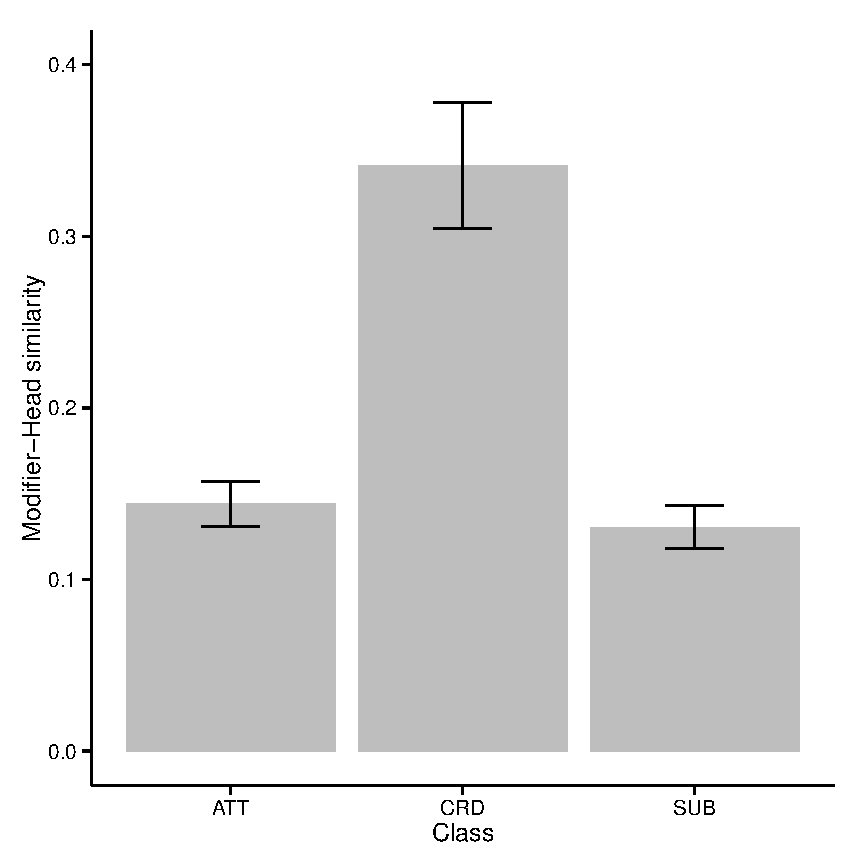
\includegraphics[width=10cm]{figures/barplot1.pdf}
\caption{Similarity between modifier and head is predictive of CRD over both ATT and SUB.}\label{fig:bar1}
\end{center}
\end{figure}


Taken together, these results indicate that the degree of semantic similarity between the compound's constituents (i.e. the modifier and the head) is a highly reliable predictor of CRD against both other classes. As shown in the barplot in Figure~\ref{fig:bar1}, the higher the similarity between the constituents, the more a compound is likely to be CRD rather than either ATT (\emph{p}=.0002) or SUB (\emph{p}=.0024). Moreover, the semantic similarity between the compound and its head is a predictive measure of SUB over both other types, as shown in Figure~\ref{fig:bar2}. That is, the more the head contributes to the meaning of the overall compound, the more the compound is likely to be SUB rather than either ATT (\emph{p}=.0355) or CRD (\emph{p}=.0146).

\begin{figure}[t!]
\begin{center}
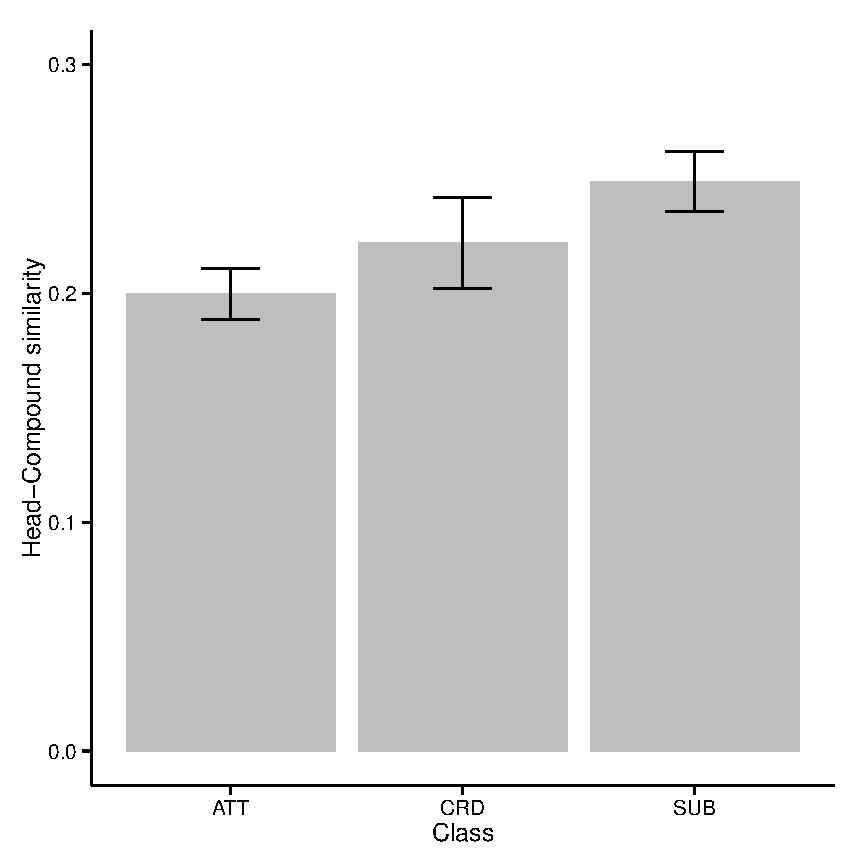
\includegraphics[width=10cm]{figures/barplot2.pdf}
\caption{Similarity between the compound and its head is predictive of SUB over both ATT and CRD.}\label{fig:bar2}
\end{center}
\end{figure}


In order to evaluate the predictive power of each model, we further computed the accuracy with which the items under investigation were correctly assigned to the correct classes. First, we obtained the classes predicted by each logit model. Second, we computed the accuracy of each model by dividing the number of correctly predicted items by the total number of items included in the final model. As a comparison, for each model we also computed the accuracy of a majority baseline obtained by simply dividing the number of cases of the majority class by the total number of cases involved.  As reported in Table~\ref{tab:qualres}, the best predictive model turned out to be the one opposing CRD vs SUB (.90 accuracy) followed by ATT vs CRD (.85) and ATT vs SUB (.61). These numbers were in line with the pattern of accuracy obtained by the majority baseline, which is sensible to the low number of CRD cases and therefore outputs higher scores for comparisons involving this class. Though our models always outperformed the baselines, the increase was noticeably lower in ATT vs SUB (+3\%) compared to both CRD vs SUB (+9\%) and ATT vs CRD (+10\%). The limited number of items do not allow us to make any statistically reliable claim on the performance of the classifier. However, our focus is on testing whether the membership in a compound class is affected by a set of theoretically-relevant variables rather than proposing an effective classification algorithm. In this light, our results provided evidence for the effectiveness of these models. At the same time, they suggested that experimenting with more data would be desirable to further validate their power.

Besides accuracy, Table~\ref{tab:qualres} reports some cases of correctly predicted and missed compounds for each of the models.

%some cases of correctly predicted and missed/omitted/unmatched compounds

\begin{table}[t]
\resizebox{\textwidth}{!}{\begin{tabular}{lcll}
\lsptoprule
Model   & Accuracy (baseline) & Predicted cases & Missed cases\\\midrule
ATT-SUB & 0.61 (0.58)     & \textit{\begin{tabular}[c]{@{}l@{}}able-bodied (ATT)\\ long-awaited (ATT)\\ schoolteacher (SUB)\\ racingclub (SUB)\end{tabular}}  & \textit{\begin{tabular}[c]{@{}l@{}}commonroom (ATT)\\ ironcurtain (ATT)\\ underbody (SUB)\\ apronstring (SUB)\end{tabular}}  \\ \midrule
ATT-CRD & 0.85 (0.75)    & \textit{\begin{tabular}[c]{@{}l@{}}best-equipped (ATT)\\ keyword (ATT)\\ father-daughter (CRD)\\ comedy-drama (CRD)\end{tabular}} & \textit{\begin{tabular}[c]{@{}l@{}}bodypolitic (ATT)\\ highschool (ATT)\\ typewrite (CRD)\\ subject-verb (CRD)\end{tabular}} \\ \midrule
CRD-SUB & 0.90 (0.81)    & \textit{\begin{tabular}[c]{@{}l@{}}comedy-drama (CRD)\\ blue-black (CRD)\\ bus-stop (SUB)\\ cutthroat (SUB)\end{tabular}}         & \textit{\begin{tabular}[c]{@{}l@{}}schoolteacher (SUB)\\ sleepwalk (SUB)\\ typewrite (CRD)\\ subject-verb (CRD)\end{tabular}} \\ \lspbottomrule
\end{tabular}}
\caption{From left to right: overall accuracy of each model as compared to the accuracy of the majority baseline, correctly predicted cases, missed cases. In brackets we report the correct class.\label{tab:qualres}}
\end{table}

\section{Discussion}
\label{sec:pez:discussion}

The present study investigated whether various, syntax-based classes of compounds (Subordinate, Attributive, Coordinate) can be described in terms of the quantitative, continuous properties of the meaning of the compounds and their constituents. To obtain these semantic measures, we generated cDSM representations for a list of compounds for which such classification was available. By running a series of logit models including both semantic and non-semantic factors as independent variables, we showed that our models are able to reliably capture different classes by means of semantic features.

\subsection{On the modifier-head similarity}

In particular, we showed that Coordinate compounds like \emph{comedy-drama} are predicted over either Subordinate (\emph{busstop}) or Attributive (\emph{halfprice}) by the higher semantic similarity between the head and the modifier. This finding is consistent with previous evidence from both theoretical linguistics and psychology. Within the lexical semantics approach, \cite{lieber5OHC} indeed proposed that Coordinate compounds are generated when the two constituents share almost identical `bodies' and `skeletons', that is, when the words to be combined have highly similar meanings.

Also, our finding is in line with several theories of conceptual combination, according to which Hybrid or Conjunctive interpretations would be produced by people for novel combinations which involve highly similar concepts, e.g. \emph{moose-elephant} (see among others \citealt{wisniewski1996}). Accordingly, and consistent with our results, Relation-linking interpretations (roughly equivalent to Subordinate compounds) would be instead produced for semantically highly dissimilar pairs, e.g. \emph{apartment-dog}. Since in our model the similarity between the constituents also distinguishes between Coordinate (Hybrid/Conjunctive) and Attributive compounds (Property-mapping), we argue that this result is consistent with the graded description proposed in many conceptual combination theories, where the difference between Property-mapping and Hybrid combinations would be due to an increasing number of both `commonalities' and `alignable differences' between the concepts to be combined \citep{wisniewski1996}.


\subsection{On the semantic role of compound's constituents}

Second, we showed that Subordinate compounds are predicted against Attributive on the basis of the higher similarity between the compound and either constituent. That is, in compositionally obtained Subordinate compounds both the modifier and the head contribute to a greater extent to the overall meaning than in Attributive ones. Moreover, the similarity between the compound and its head is a reliable predictor of Subordinate over both other classes.

First of all, these findings are again consistent with the lexical semantics literature \citep{sbg2005,lieber5OHC}. In it, Subordinate compounds are typically characterized by a structure in which the head \emph{selects} its argument. Therefore, the head contributes more to the overall meaning in this kind of compounds compared to the other classes, where a formal relation between the elements is absent. Also, these results are consistent with the different mechanisms proposed in the conceptual combination literature for Relation-based interpretations (capitalizing on a `slot-filling' procedure) and Property-based ones (where an `alignment' process is routinely carried out) \citep{wisniewskigentner,wisniewski1996}. In a nutshell, the slot-filling procedure would imply a bigger role of the compound \emph{head} compared to the other competing mechanism since, during combination, the head would be just \emph{filled} in one of its `slots' by the modifier concept.

Interestingly, these findings are also consistent with evidence from embodied cognition \citep{louwerse2008}. In particular, the embodied conceptual combination theory ({ECC}o) by \cite{lynott2009} proposes that the great majority of relational interpretations (corresponding to Subordinate compounds) are `non-destructive', namely, they result from the combination of constituent concepts that are left intact during the meshing of their `affordances'. To illustrate, in this approach the compound \emph{picture book} (i.e. `a book that has pictures’) is non-destructive, since the \emph{pictures} in question are still intact entities in the pages of the \emph{book}. Simplifying somewhat, the combinatorial procedure that leads to Relation-based interpretations (Subordinate) does not modify heavily the meaning of the original constituents, whereas Property-mapping ones (Attributive) are almost always destructive, that is, they involve the `destruction' of (part of) the constituent concepts. Using an example from \cite{lynott2009}, the compound \emph{icicle fingers} would reduce \emph{icicle} to a representation of `coldness' and `stiffness'. At the same time, the representation of the head (\emph{fingers}) would be switched toward a more figurative, metaphorical meaning, less similar to its prototypical representation (see also, e.g., \emph{iron curtain}). In this light, the similarity between either constituent as an independent word and the compound will be generally higher in Relation-based (Subordinate) compared to Property-based interpretations (Attributive), given that the combinatorial procedure of the former type does not heavily modify the meaning of the original constituents. Moreover, this observation provides indirect evidence that meaning representations extracted from texts via distributional semantics models can encode grounded information, at least to some extent \citep{louwerse2011}.

\subsection{On attributive compounds}

Third, compositionally-derived Attributive compounds are characterized by both a weaker contribution of the constituents in determining the overall meaning compared to Subordinate and a lower similarity between the constituents compared to Coordinate. This pattern of results is again consistent with \cite{lieber5OHC}, who proposes that Attributive formations emerge when the semantic
features of the constituents are too disparate to be interpreted in a Coordinative way and lack the argument structure that is typical of Subordinate compounds. Accordingly, Attributive compounds would represent a last-resort strategy used when the typical semantic features of the other classes are not satisfied \citep{lieber5OHC}. This description, according to which Attributive compounds would result when no discriminative features are present, is in line with evidence from conceptual combination showing that acceptability judgements for Property-based (Attributive) interpretations to novel compounds (e.g., a \emph{whale boat} is `a large boat’) are slower compared to Relation-based (Subordinate) interpretations (e.g. a \emph{whale boat} is `a boat for hunting whales') \citep{gagne2000}. According to \cite{gagne2015}, indeed, this would suggest that Relation-based interpretations are the product of an initial compositional process that, in the absence of the features that lead to either a relational interpretation (Subordinate) or a coordinate interpretation (Coordinate), leads to Property-mapping interpretations.

\subsection{On the methodology}

On the methodological level, it should be mentioned that we used a compositional model to generate representations for a list of compounds whose constituents were nouns, verbs, adverbs, adjectives, etc. even though in the training phase only noun-noun compounds from CELEX were used. This could have represented a weakness for the system, causing the model to be biased toward noun-noun combinations. By looking at the results, however, we observed a similar, remarkably good performance of the model in all items, regardless of the grammatical category of the constituents. This is also clear by inspecting the examples in Table~\ref{tab:qualres}, where it can be noted that the parts-of-speech are almost uniformly distributed. However, it might be still possible that a richer training set might lead to even better results, perhaps achieving a better performance in generating meaning representations for less systematic, more opaque compounds. Indeed, we hypothesize that the lower accuracy obtained by the model opposing Attributive vs Subordinate compared to the others might be possibly due to this issue. Finally, we believe that the effectiveness of such an approach might be further validated by testing it on a larger (and possibly balanced with respect to compound type) set of annotated compounds. This, on the one hand, would strengthen the predictive power on the prediction task. On the other hand, it would allow more extensive, fine-grained analyses on the successes and failures of the models. We plan to further investigate this issue in future work.


\subsection{On the effectiveness of cDSMs in predicting compound relations}


The effectiveness of our approach in the proposed task is in line with previous work showing that compositional models of distributional semantics are successful in capturing relational information between the constituents of a compound. In particular, our task is related to that of predicting compound semantic interpretation (see section~\ref{sec:relnew}), where compositionally-obtained representations have been used to assign the correct semantic relation to noun-noun expressions. By experimenting with a number of cDSMs (including the one adopted in this study by~\citealt{guevara2010}), for example,~\cite{dima2016compositionality} obtained results comparable to state-of-the-art in 2 popular datasets~\citep{o2007annotating,tratz2010taxonomy}. Compared to SoA methods, however,~\cite{dima2016compositionality} only exploited information from word embeddings, thus proving the effectiveness of both distributed representations and compositional methods. In quantitative terms, our results are not directly comparable due to both the different experimental setting (we did not tackle the task as a classification problem) and the number of relations involved (3 vs either 6 or 43). Moreover, our results cannot be compared with previous work since, to our knowledge, we are the first in proposing this task. However, these studies jointly show that compositional  representations are successful in predicting compound relations defined on either \emph{semantic} or \emph{syntactic} bases.


\subsection{Final remarks}

In conclusion, this study suggests that different compound types identified on syntactic bases can be also defined in terms of continuous, quantitative features of the meaning of the compound and its constituents. We believe that discrete and continuous approaches are two faces of the same coin, the former representing a theoretically motivated, cross-linguistically valuable framework aimed at describing complex linguistic phenomena, the latter providing an interesting way to quantitatively test them. As indicated by our results, compositional models of distributional semantics present a flexible and powerful way to capture many of these phenomena.

%\section*{Abbreviations}
\section*{Acknowledgements}
We are grateful to Marco Baroni and Laura Vanelli for their valuable feedback during the early stages of the project. We thank Sergio Scalise for providing the MorBoComp subset used in the experiment. We are also grateful to the participants of the First Quantitative Morphology Meeting (Belgrade, July 2015) for the helpful questions and discussion.


{\sloppy\printbibliography[heading=subbibliography,notkeyword=this]}

\end{document}
